
\begin{problem}
Determine which of the following two graphs are planar.
Justify your answer. (You need to either show a planar embedding or
use Kuratowski's theorem.)

	\begin{center}
		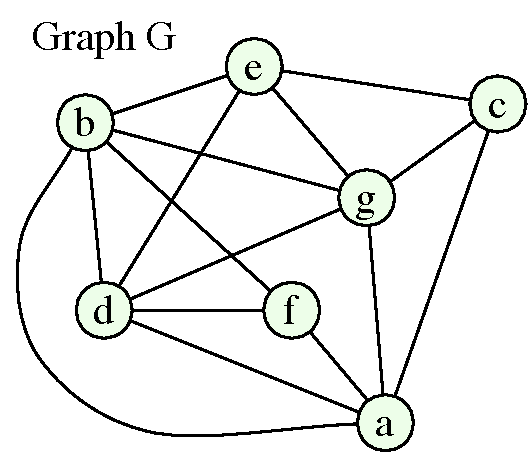
\includegraphics[width = 2.3in]{graphGa_hw5.pdf}
		\hfill
		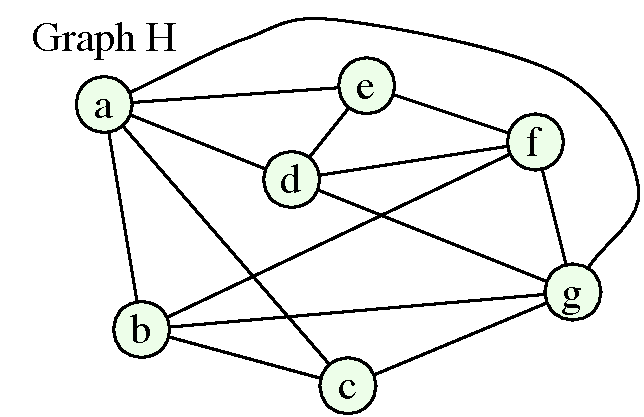
\includegraphics[width = 2.8in]{graphHa_hw5.pdf}
	\end{center}

\end{problem}

\begin{solution}
Graph $G$ can be shown to be nonplanar by merging $a\to f$ and $c\to e$.

\begin{center}
  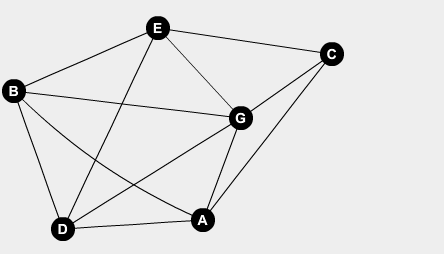
\includegraphics{amergef.png} \\
  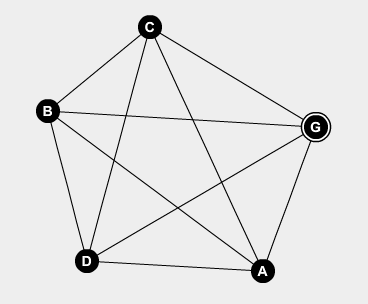
\includegraphics{cmergee.png}
  \end{center}

The above is the complete graph $K_5$. By Kuratowski's theorem, $G$ containing $K_5$ shows that it is nonplanar.

\bigskip
\bigskip
\bigskip

Graph $H$ can be shown to be planar with rearrangement.

\begin{center}
		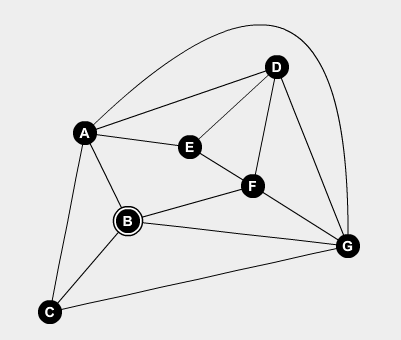
\includegraphics{graphh.png}
\end{center}

Since there are no intersections, $H$ must be planar.
\end{solution}
%%%%%%%%%%%%%%%%%%%%%%%%%%%%



